\section{Introduction}
\label{sec:Introduction}

With widespread use of social medias, such as blogging services or social
network services (SNS), today we have become able to publish information
on the Web more easily than previously.  Especially recently,
microblogging services have been growing explosively.

Microblogs are a new type of services which have both characteristics of
blogs and SNS.  In microblogs, users can post short messages more easily
and rapidly than in conventional blogs or SNS.  Microblogs are not
necessarily regarded as a medium for publishing useful information to
the public, so users of microblogs post messages more casually than that
of conventional blogs or SNS.  Because of these characteristics, a large
number of messages are posted on microblogs every day, and the messages
contain various types of contents, from personal notes or life logs to
useful information or discussion on specific topics. Furthermore,
messages describing current situations especially characterize
microblogs among various types of messages.  This type of message is
much more frequent than in conventional blogs or SNS, so a large number
of microblogging messages include real-time information.

Among many microblogs,
Twitter\footnote{\url{http://twitter.com/}} is especially growing
rapidly.  As of 2012 December, Twitter has over 200 million active users
in the world\cite{TwitterUsers}, and as of June, more than 400 million
messages are posted on it per day\cite{TweetsPerDay}.  In Twitter, users
can post short messages with at most 140 characters, which are called
tweets.  By this limitation, Twitter makes information publishing more
easily and rapidly than conventional blogs or SNSs.  The
most distinctive feature of Twitter is its mechanism of
\emph{''follow''}.  In Twitter, if a user follow other users, all tweets
by these followee users are retrieved in real time, and are shown in a
list sorted in the reverse chronological order, as shown in
Figure~\ref{fig:twitter}.  This list is called the \emph{''timeline''}
of the follower users.  The mechanism of follow is more casual than
user-linking functions in ordinary SNS; it does not require the
permission by the followee, and does not necessarily imply reciprocal
relationship. Another important function in Twitter is the
\emph{''reply''} function, by which a user can post a message as a reply
to another user.  By using this function, users can use Twitter for
conversation, as in instant messaging services.

{\footnotesize
\begin{figure}[t]
\begin{center}
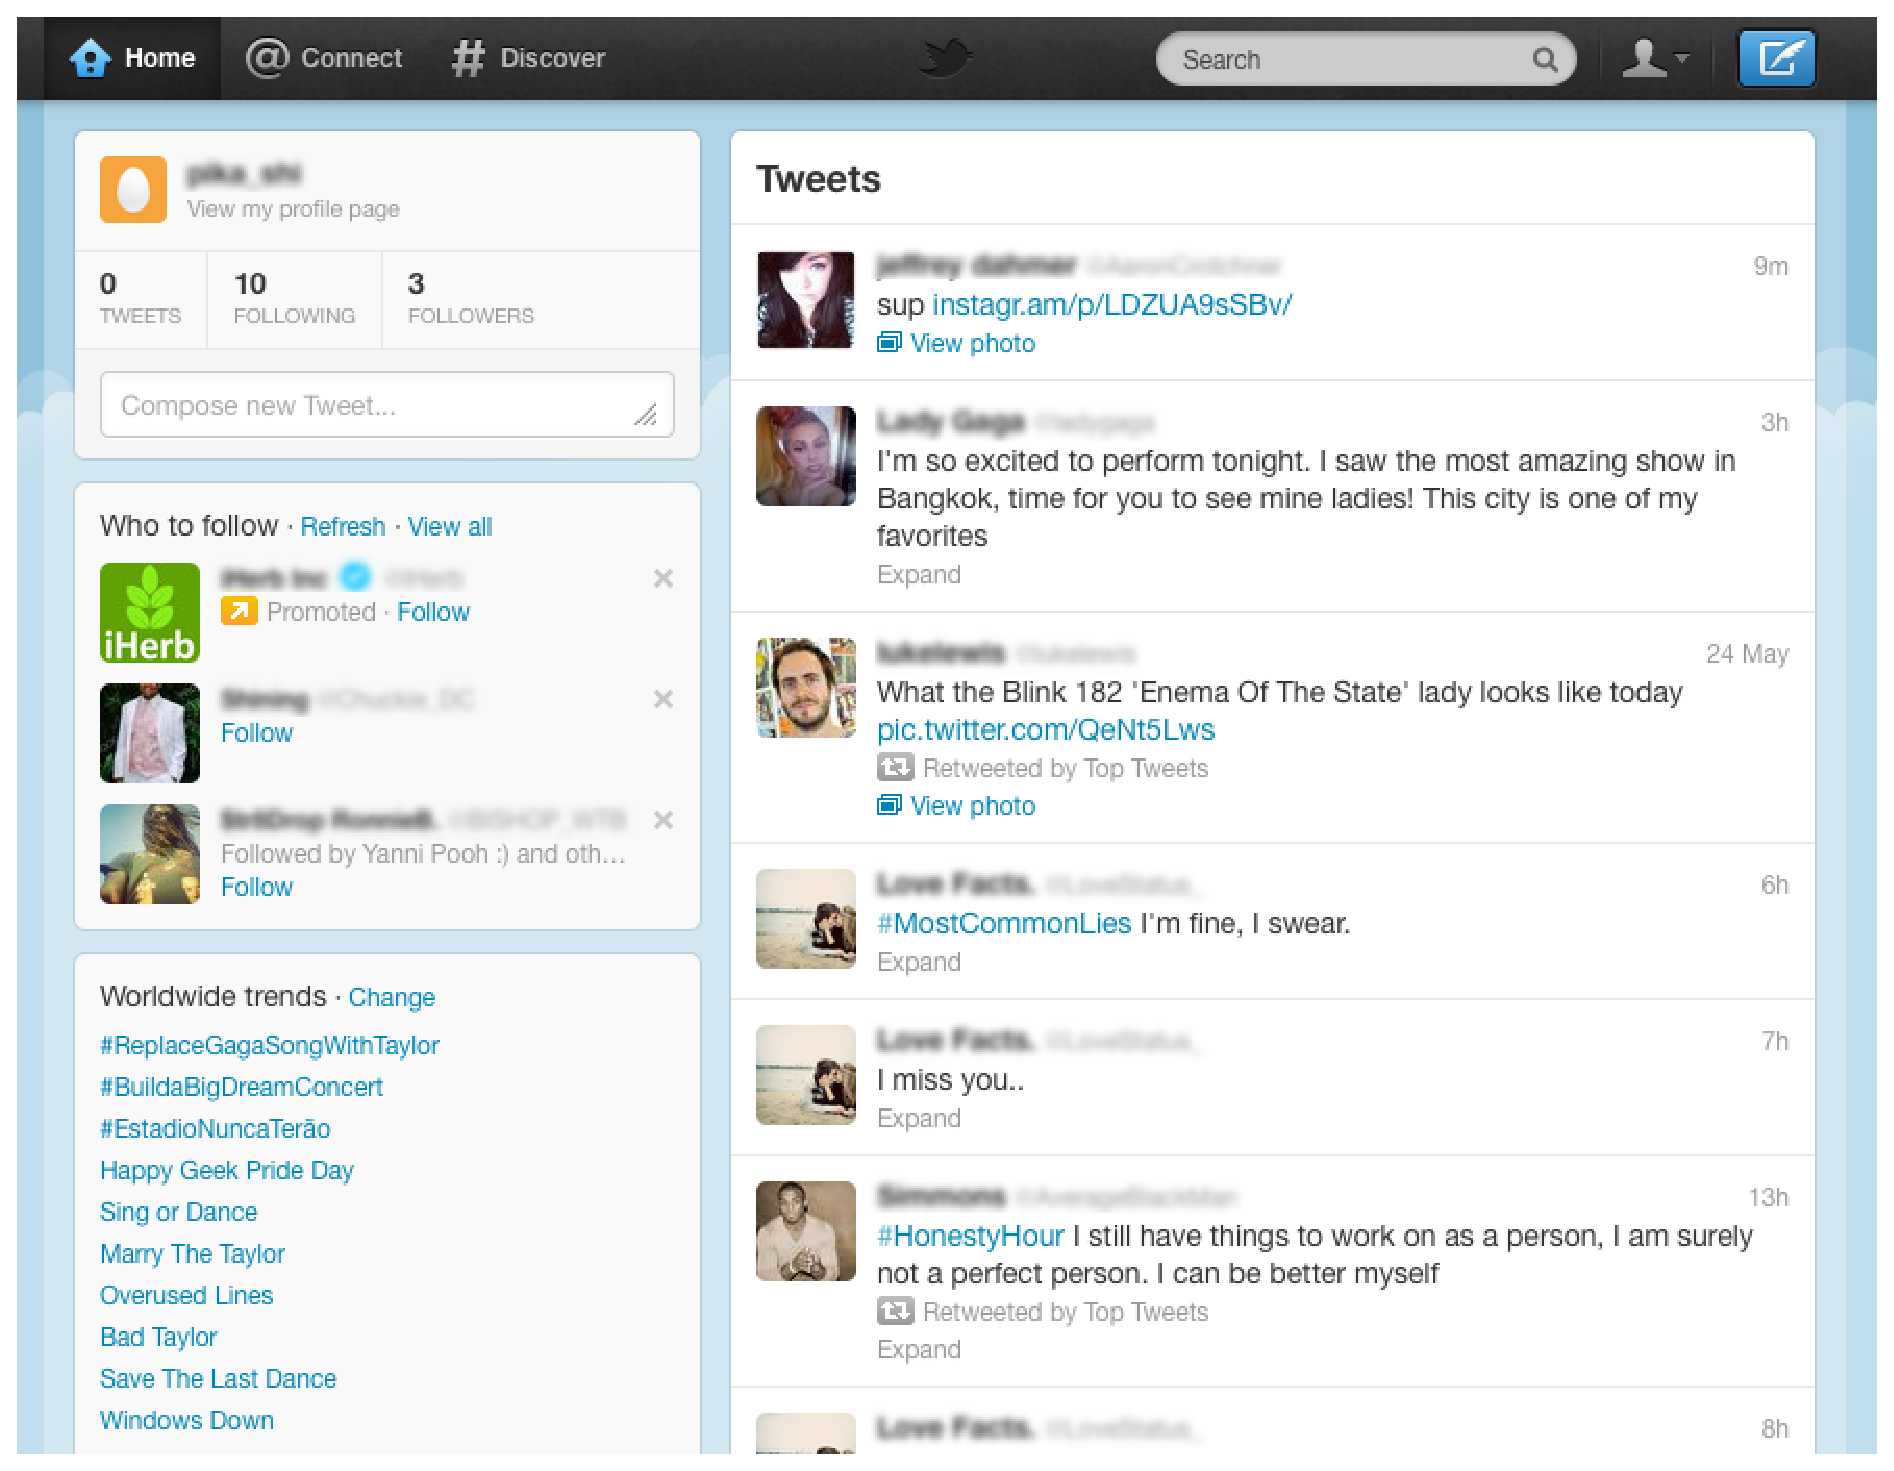
\includegraphics[width=14cm]{images/screen_shot.eps}
 \caption{An example of a user's timeline in Twitter}
\label{fig:twitter}
\end{center}
\end{figure}
}

Twitter has many characteristics of conventional social medias, so it is
used for many purposes.  Some publish information to the public widely,
some publish information specified for certain topics, and some
communicate with their friends or others.  Because of this
characteristic, Twitter has attracted great attention as a new type of
social media.

As explained above, Twitter is used for various purposes.  As a result,
the wideness of target scope of information publishing varies greatly
among users.  So, in this study, we propose a method to classify
Twitter users from the point of view of how widely target scope of
their information publishing is, i.e., whether they publish information
to the public widely or publish information specified in certain users.
In this study, we call the former \emph{``target specificity is
low''}, and the latter \emph{``target specificity is high''}. In this
method, we
focus on the followers of the user, and we classify him/her
whether his/her followers are consistent in some noticeable characters
or not.  If his/her followers are consistent in some noticeable
characters, it suggests that he/she publishes information in which
particular users are interested. On the other hand, if they are not
consistent in any noticeable characters, there is a high
probability that the user is followed by a wide variety of users and it
suggests that he/she publishes information in which the public, i.e.,
almost all users, is interested.

In addition, in this study, we focus on Twitter users classified into
``target specificity is high'' by the above, and we propose the
method to determine what causes their target specificity, i.e., why
their target scope of information publishing is specified to certain
users.  In a large number of Twitter users, their target scope are
specified to certain users, and the causes vary from user to user.  For
example, users publishing technical information about programming is supposed to
publish information to unspecified users, but their target specificity
is considered high because the topic of their publishing information
is specified to certain users, who are
interested in programming.  And also, users communicating with
their friends or who announces to club members is supposed to publish
information to the users specified
extensionally. So their target specificity is supposed to be high,
regardless of contents of their publishing information.  In this method,
first, we roughly classify causes of the target specificity into two
categories: (1) because they publish information specified for certain
topics, and (2) because they publish information to the users specified
extensionally. Then we construct classifiers which determine
whether users only belong to the category (1), only belong to the category (2),
or belong to both (1) and (2), based on various features which correlate
with each category.  Figure~\ref{fig:Flow} shows the overall flow of our
methods.

{\footnotesize
\begin{figure}[t]
\begin{center}
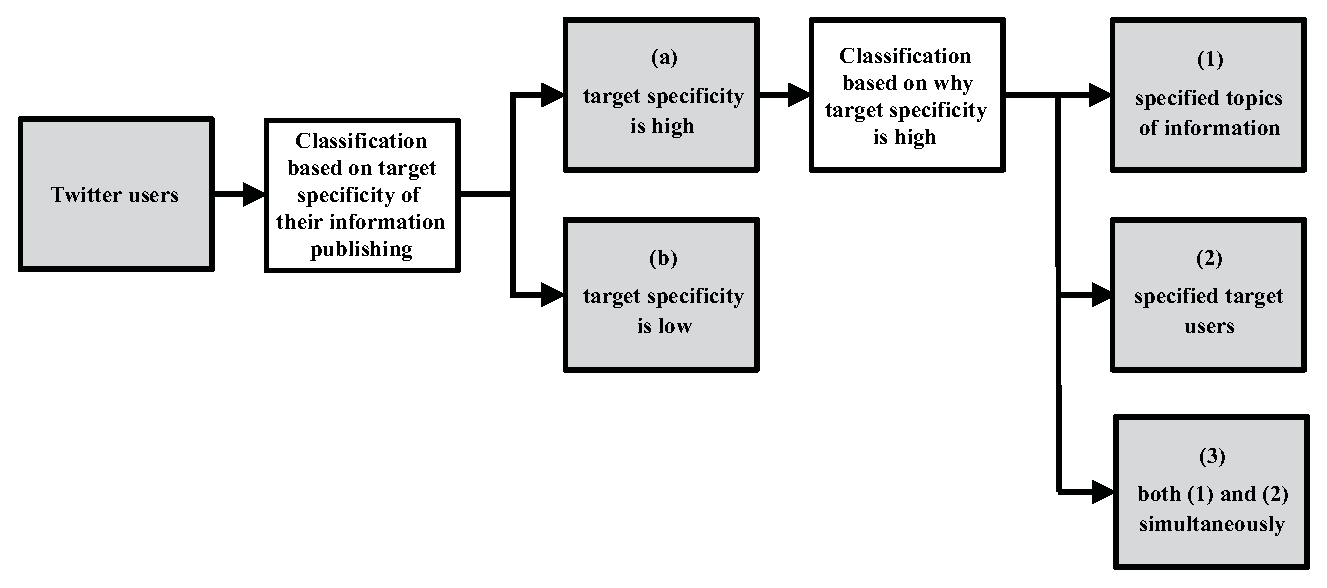
\includegraphics[width=14cm]{images/flow.eps}
 \caption{Overall flow of our methods}
\label{fig:Flow}
\end{center}
\end{figure}
}

On the Web, it is hard to know what kinds of users each Web page targets
to.  But in Twitter, we can know what kind of users each user target to
by their follow relationships.  By using this relationships, we can
classify users based on the target specificity of their information
publishing.

Twitter user classification of this study is supppsed to apply to
Twitter search.  In current Twitter search, we input a search word in the
search box and receive messages including the word.  But with this
method, messages in search results have various target scope of
information publishing.  So it frequency happens that messages of
certain target scope we need are buried in many other messages. For
example, when we search in Twitter with the word ``MacBook
Air'', what kinds of messages we needs depends on the situation of
that time, e.g., we may need public news about MacBook Air, we
may need technical information about it, or we may need
users' reviews of it to refer when we buy new one.  But in
current Twitter search, these information is mixed up in search results.
At that time, by using the classification of this study, we can
search messages based on what kinds of users they target to.  In this
way, we can prevent messages we need from being buried in many other
messages and find messages we need easily.

The contribution of this paper is summarized as follows.

\begin{itemize}
\item We propose a new classification scheme of Twitter users' target
      specificity of information publishing.
\item We show a method of classifying users based on above scheme.
\item In regard to users classified into ``target specificity is high'',
      we show a method of determining why their taiget specificity is
      high.
\end{itemize}

The rest of this paper is organized as follows.  Next section explains
some related work and makes the position of this study clear.  Then we
define Twitter users' target specificity of information publishing and
formulate our problem, and we discuss why their target specificity is
high in \ref{sec:Target Specificity}.  In
\ref{sec:ClassificationMethod1}, we explain the method of classifying
Twitter users based on their target specificity of information
publishing.  In addition, in regards to Twitter users
classified into  ``target specificity is high'' by the above method,
we explain the method of determining why their target specificity is
high in \ref{sec:ClassificationMethod2}.  Then in \ref{sec:Experiment},
we presents the results obtained from experiments we conducted to
evaluate our methods.  \ref{sec:Conclusion} concludes the paper.

